\chapter{Detection of cells \status{new}}
	\label{chap:cell_detection}
	\section{Overview \status{new}}
	
	what it does
	
	that is laerns from datasets which is required to make it robust in noisy datasets
	
	that it is mostly Arteta's work, with some moditications to make it run faster
	
	\section{Learning to detect non-overlapping cells \status{new}}
		\rewrite{Several of these subsections are directly taken from Arteta's paper. They are mean as guidance, but should be adapted appropriately.}
		
		\todo[inline]{Check both Arteta's papers on the subject}
		\todo[inline]{Subsection with the changes that were made to Arteta's work}
		\subsection{Extremal regions \status{new}}
		
		what are extremal regions and that they are obtained from the MSER featre detector
		
		why are they good: fast, robust to contrast and to what else
		
		what is their work in the detector: they are candidates cells, that are then evaluated as cell/nocell	
		\subsection{The non-overlap constraint \status{new}}
		
		What it means: we cant detect overlapping cells
		
		why is that ok: the datasets don't exhibit such behavior. much more training data would be required, which means more annotations.
		
		\subsection{Formulation of the model \status{new}}
		
		????
		
		\subsection{Learning the model \status{new}}
			
			\todo[inline]{Info about the binary/structural classifier}

		\subsection{Implementation details \status{new}}
			\subsubsection{Dynamic programming for inference \status{new}}
		\subsection{Summary \status{new}}
		
	\section{Speeding up the algorithm \status{new}}
	\todo[inline]{review this section}
	The main drawback of the algorithm presented by Arteta \cite{arteta12} is the poor performance. The original algorithm took about 30 seconds to detect cells in a 400x400 image. Because we will be processing hours of microscopy video it was important to reduce the detection time as much as possible.  The major performance improvements where achieved by addressing three things.
	
	The algorithms needs to extract a set of feature on every single detecetd MSER. First, we have first fine-tuned the MSER detector to detect less cells, more robustly.
	
	Second, we have identified features that are slow to compute and improved their algorithmic behaviour. One such feature is the Contour Points Distribution Histogram implemented in \textit{cpdh.m}. The function was performing excessive calls to slow functions to extract region characteristics, and was rewritten to call these function less often, without affecting its value.
	
	Second, several MATLAB builtin function were modified to remove excessive parameter checking, which in several cases represented an overhead of over $30\%$. These parameter checks are welcome when developing the algorithm, but once the algorithm is complete, several of these checks can be safely removed. \rewrite{Not sure I can write this, since the matlab code is copyrighted}
	
	These opimizations resulted in a significant performance boost. Instead of 30 seconds, the algorithm can now detect cells on the same images in about \todo{Measure the number of seconds it takes to process one of these 400x400 images}.
	
	\section{Feature selection \status{new}}
	
	The effictiveness of the machine learning method to detect cells depends on the quality of features. Good features have a lot of discriminative power between cells and non cells. The used approach classifies extremal regions as cell/non-cell. The regions are extracted using the MSER detector. Then each region is processed and features are extracted from it. We have evaluated several combinations of these features:
	
	\begin{enumerate}
	    \item the area A of the region represented by a 10-dimensional binary vector with the entry $\lceil log A \rceil $ set to 1.
		\item 10-dimensional histogram of intensities within the region
	    \item the position of the descriptor in the image in terms of x-y coordinates of a centroid fitted to the descriptor.
	    \item two 6-dimensional histograms of differences in intensities between the region border and a dilation of it for two different dilation radii
	    \item a shape descriptor represented by a 60-dimensioal histogram of the distribution of the boundary of the region on a size-normalized polar coordinate system
	    \item The orientation of the descriptor after attempting to normalize its orientation
	    \item The proportion of edge-pixels in the region.
	\end{enumerate}
	
	Each of these features has different discriminative power, and takes some time to compute. The application of the cell detector requires that images are processed within a time limit. For this reason, we have trained and tested the algorithm with all the $2^7 - 1$ possible combinations of these features.
	
	We have also developed a function that helps select the most appropriate set of features given specific constraints, for example a maximum computation time, minimal precisiona and recall values, etc. A graph generated by the function is shown in figure \ref{fig:bestFeatureSelector}.
	
	\begin{figure}
		  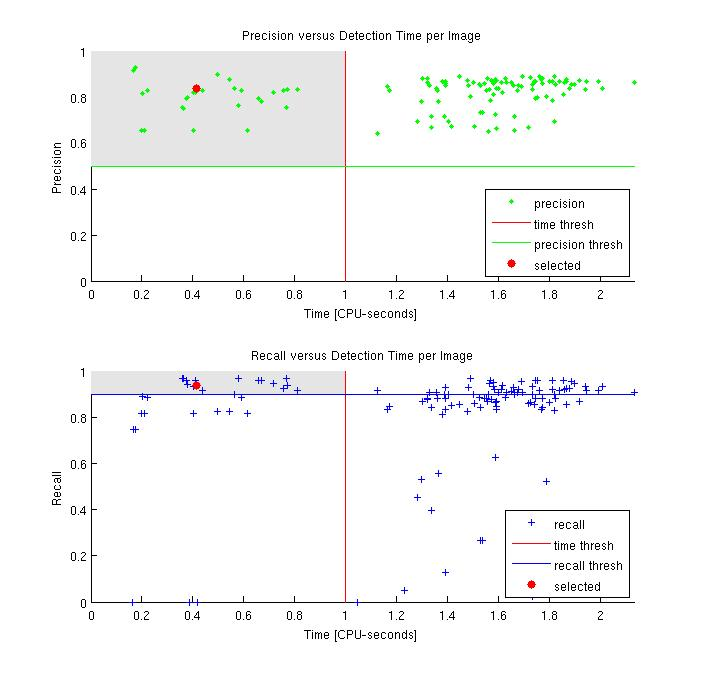
\includegraphics[width=\textwidth]{images/best_features}
		\caption{The plots helps the user to select the most appropriate feature, given a combination of computation time per image, mean precision and recall. This example, which was obtained by selecting only within feature sets that compute in less than 1 CPU-second, have at least 0.5 precision and 0.9 recall have resultsed in a feature set containing features 1, 3 and 4. Most importance was given to precision followed by computation time and recall. The selected feature set computes in 0.414 cpu-seconds (Intel(R) Core(TM) i7-2600 CPU @ 3.40GHz) per image, with mean precision of 0.836 and mean recall of 0.9363.}
	    \label{fig:bestFeatureSelector}
	\end{figure}
	